\section{Introduction}

\todo{Bitte noch anpassen falls euch der Wortlaut net so passt}

Mobile Apps get used for quite literally everything in today's World. So after
we noticed that there is no application that allows the efficient planning of
campaigns like the "Sternsinger-Aktion" we asked ourselves why, and furthermore,
how hard it would be, to create an App with intuitive Usability for the sole
purpose of simplifying the process of managing such a campaign and gaining a
general overview of the progress made. \newline

\todo{Vielleicht noch kürzen, wirklich nur die groben Themen?}
The research part of this thesis will be dedicated to how components should act
and look, so that new users can use this tool without requiring a long "onboarding" phase. It should feel familiar to interact with elements and the
borders of what users can and can't do need to be clearly defined. Because our
application also needs a somewhat reliable data source to guarantee the
consistency and accuracy of marked addresses in our app. For this purpose we
researched ways to keep our database up-to-date, without the need of much manual
intervention. After defining the projects requirements, we noticed that we need
to somehow calculate which addresses are "Border" addresses. So we decided to take a look into different algorithms for this task and compare them concerning their efficiency and then decide on one of them and implement it.
\newline


This thesis contains an in-depth description of our thought and development
process, as well as any other steps we took to achieve our goal of a
functional mobile application that can be used by volunteers in course of the
"Sternsinger-Aktion 2025" taking place in the parish of Lieboch. \newline

\todo{Wortwiederholung austauschen}
The result of this thesis should be a mobile app that provides users with the addresses that they need to visit on this day. They then should be able to easily mark the houses they already visited. If something unusual happens at this address, the user should be able to take note of this, so the organizers have knowledge of it and can account to it in the following year.

\newpage

\subsection{Team}


This thesis was created by three Students attending the BHIF20 at the
HTBLA Kaindorf Computer Science Department.\newline

\todo{andis bild anpassen }

\begin{center}
    \begin{tabularx}{\textwidth}{X X X}
        \centering
        \textbf{\daAuthorOne} \newline
        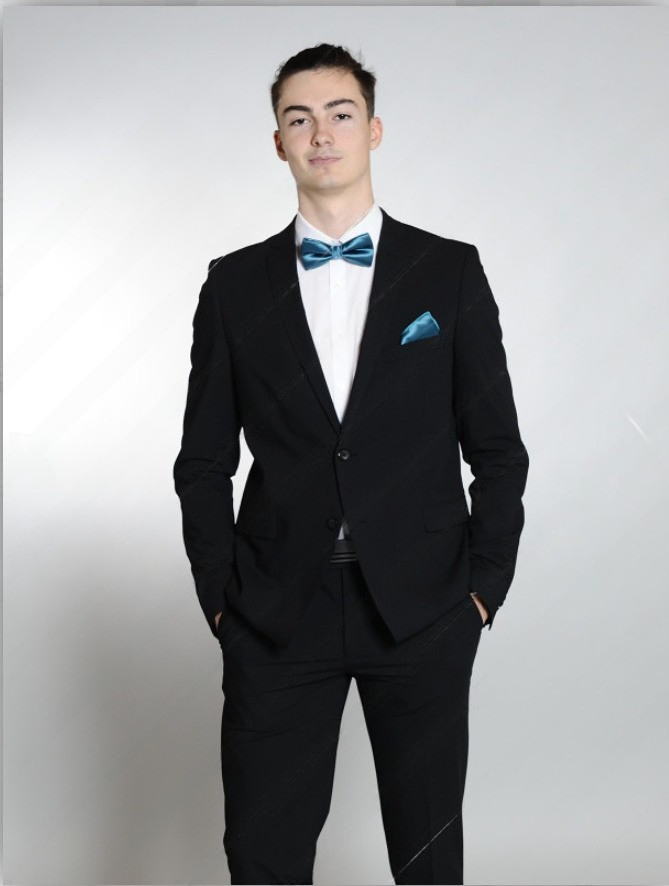
\includegraphics[width=0.28\textwidth]{images/people/leonEdlinger.jpeg} \newline
        Database, Admin-Panel &
        
        \centering
        \textbf{\daAuthorTwo} \newline
        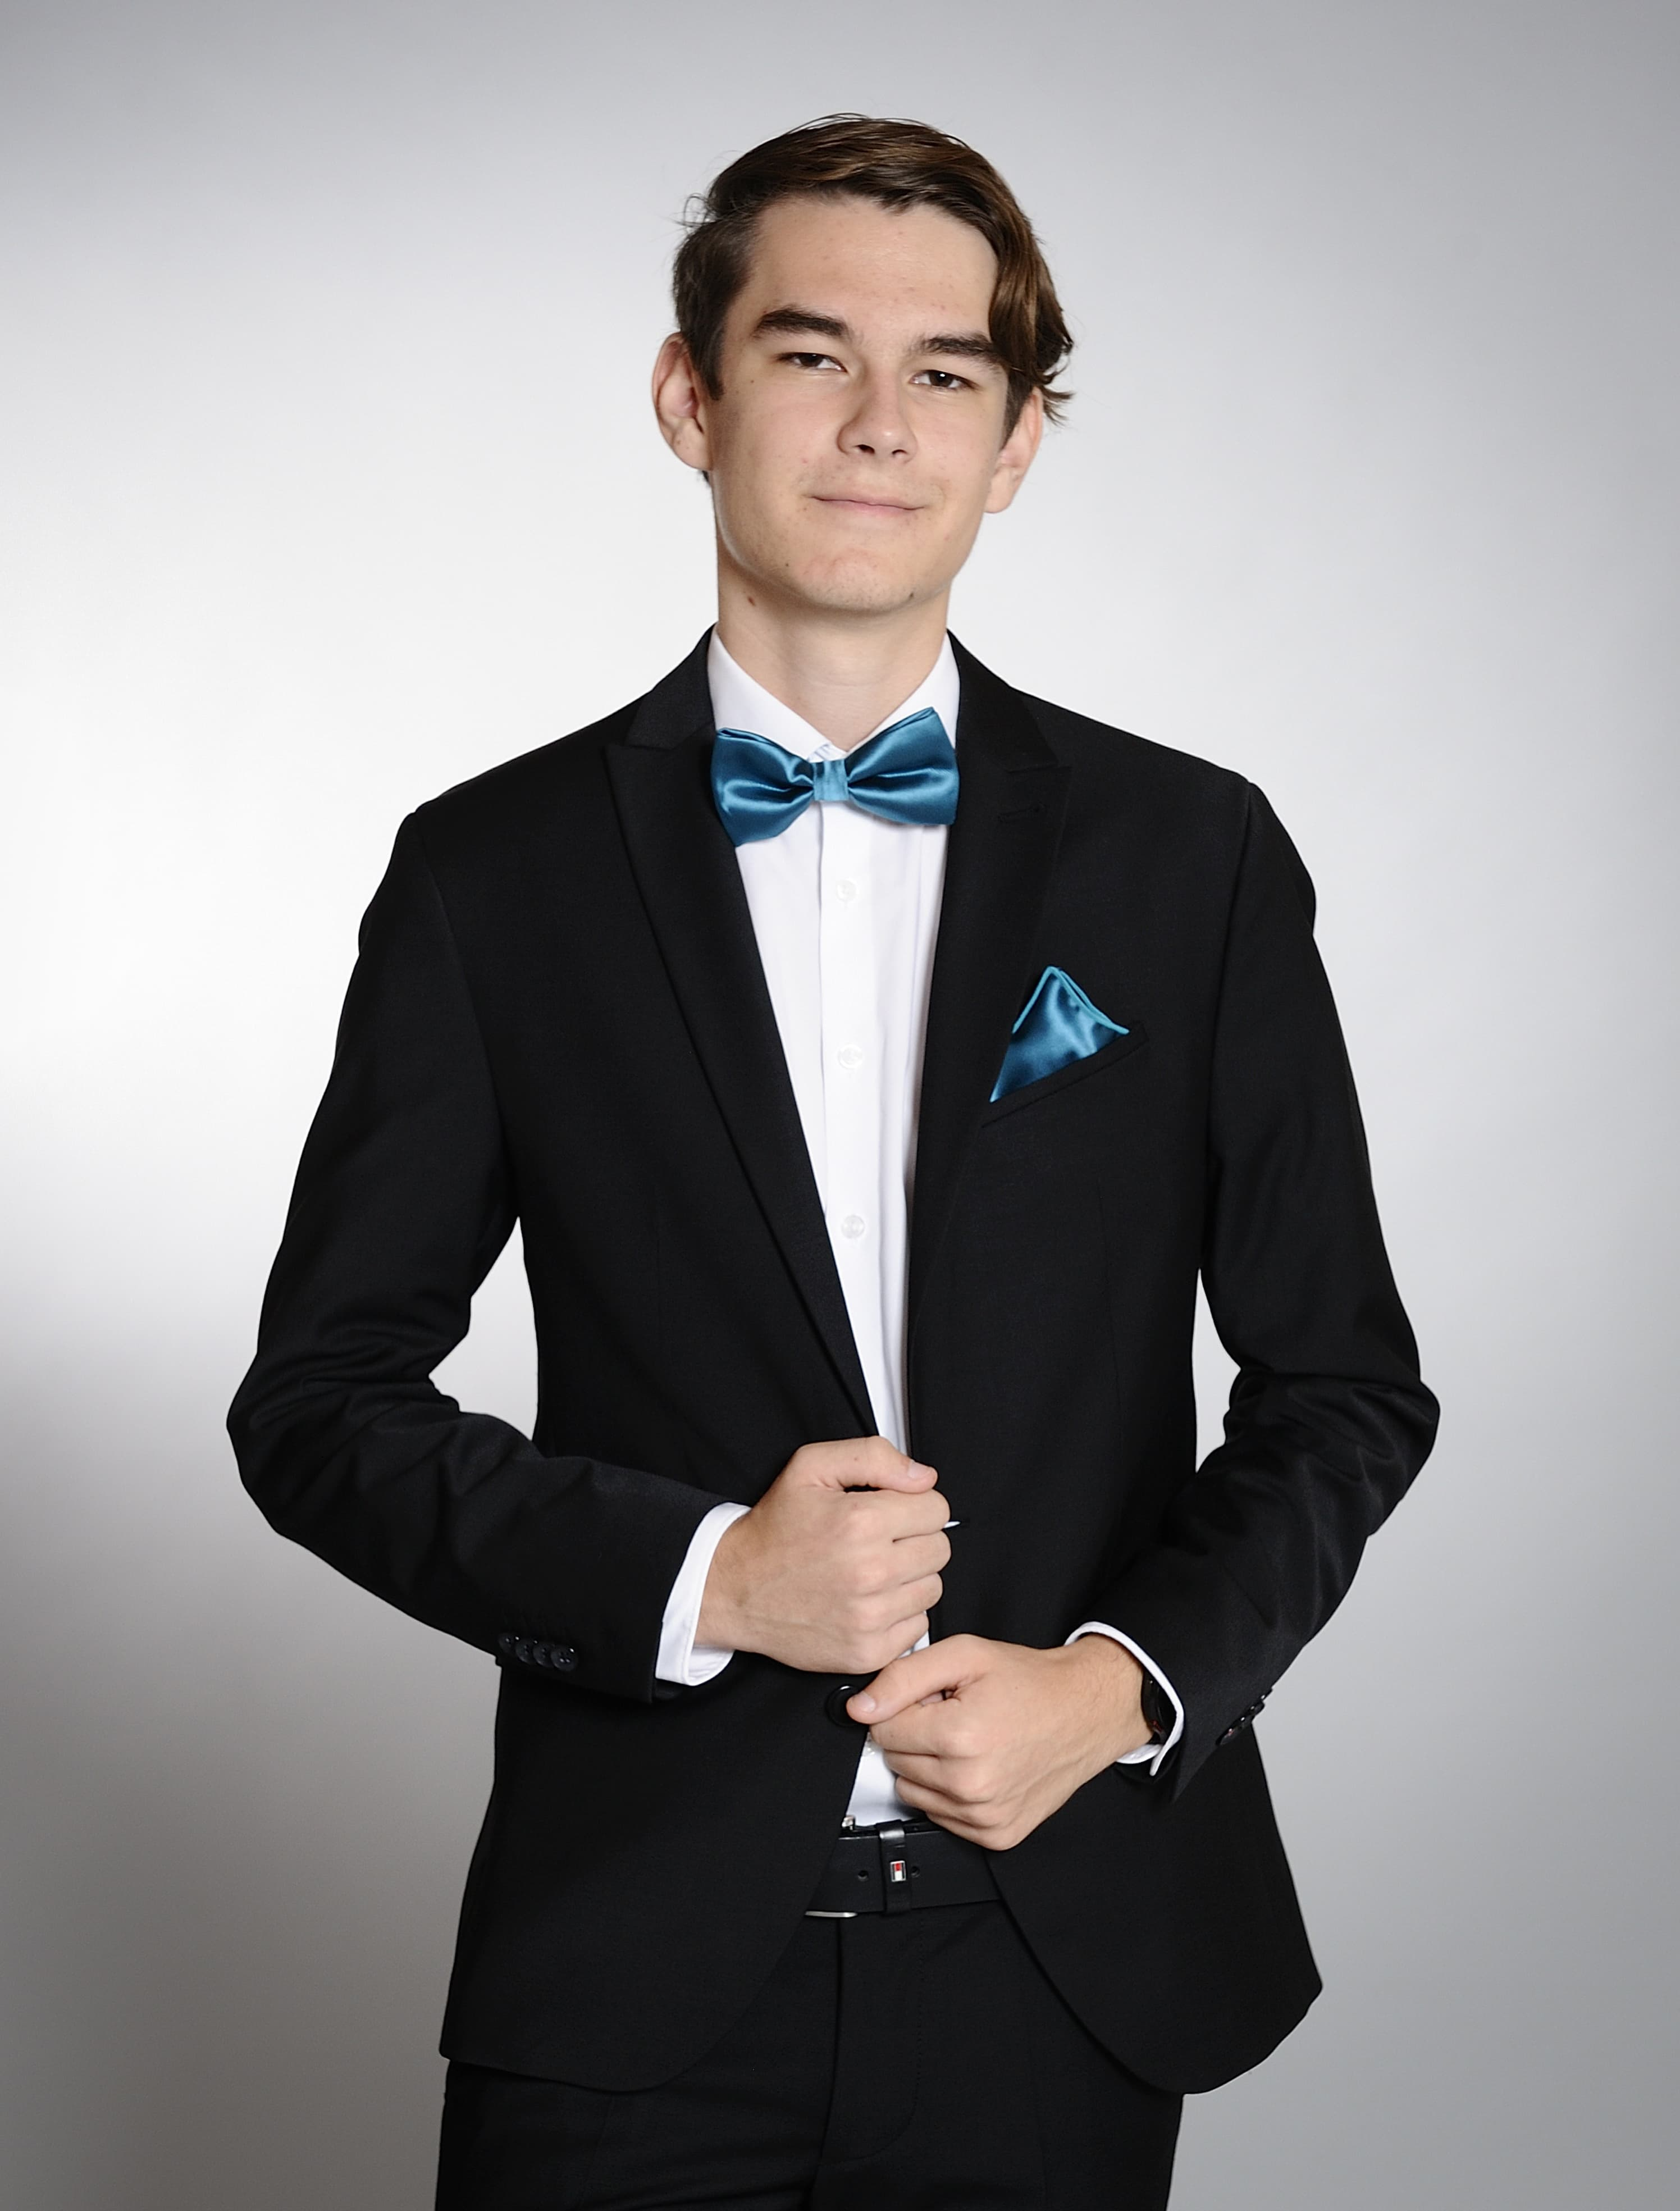
\includegraphics[width=0.28\textwidth]{images/people/paulGigler.jpeg} \newline
        Deployment, Mobile App &
    
        \centering
        \textbf{\daAuthorThree} \newline
        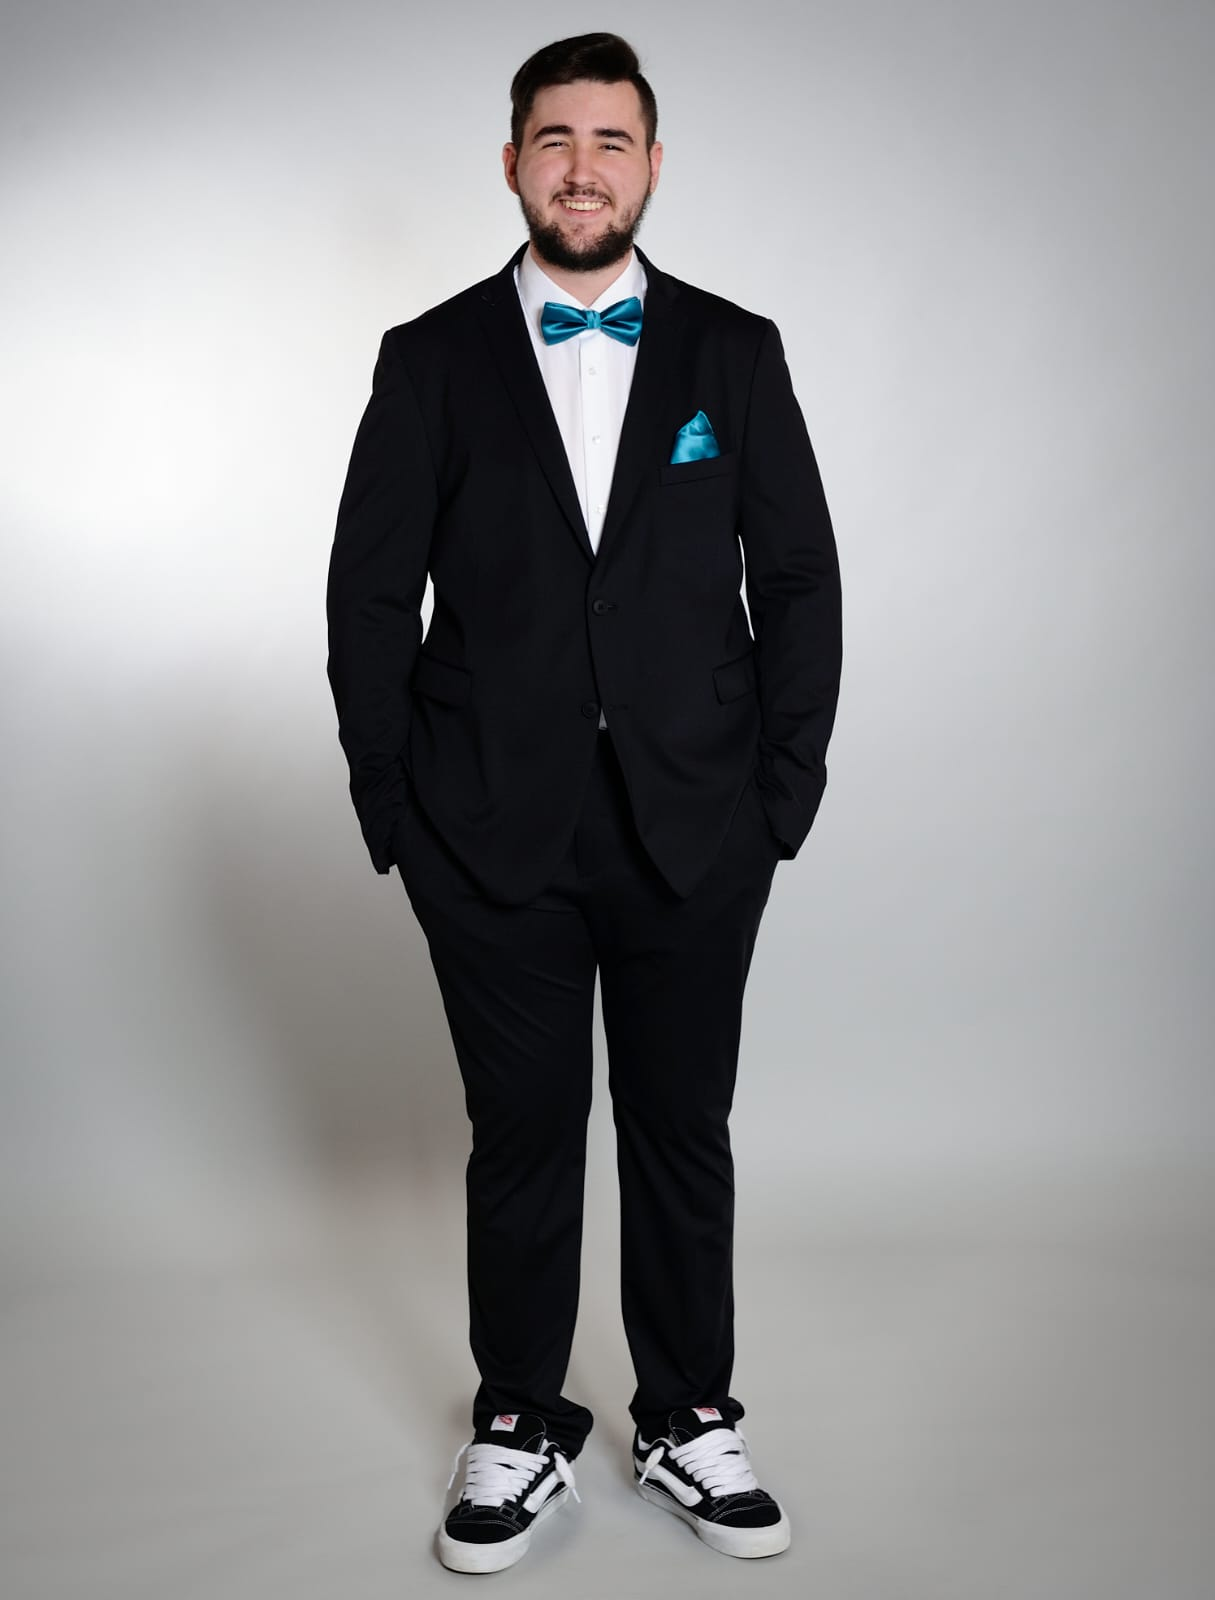
\includegraphics[width=0.28\textwidth]{images/people/andreasWeissl.jpeg} \newline
        Backend
    \end{tabularx}
    \end{center}
\subsection{Motivation}

\newpage